\section{Introduction}

Generalist robot policies increasingly use vision-language-action (VLA) architectures to map visual observations and natural-language instructions to continuous robot actions. This formulation promises broad skill coverage, but it inherits a structural property of real robot data: demonstrations are not uniformly distributed. Everyday tasks such as picking and placing common objects are frequent, while rare object-relation combinations may appear only a few times.

Long-tailed imitation learning differs from long-tailed image classification in a crucial way. The model is not only choosing a class label; it must produce a temporally coherent action sequence conditioned on a language instruction, object layout, and robot state. A rare task failure can therefore arise from several sources: insufficient exposure, poor spatial grounding, weak object binding, or interference between semantically adjacent tasks. Simply increasing the sampling frequency of rare demonstrations may not create the missing spatial or action diversity.

The first long-tailed robotic imitation benchmark, Beyond the Majority~\cite{zhu2026beyond}, makes this issue concrete. It constructs \liberocorelt{} from LIBERO tasks, with the steep task-frequency profile shown in Figure~\ref{fig:intro_longtail}, and shows that conventional re-sampling barely improves the miniVLA baseline. The paper diagnoses a large increase in target-approach failures under long-tailed training and proposes Approaching-Phase Augmentation (APA), which transfers head-task approaching trajectories to tail objects. APA is an important first step, but it also leaves open a more general question: can we improve rare-task policies without synthesizing new positive trajectories or depending on a particular phase decomposition?

\begin{figure}[t]
  \centering
  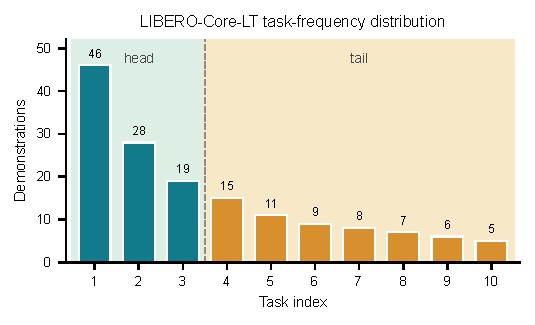
\includegraphics[width=0.56\linewidth]{figures/rbtad/fig1_intro_longtail_distribution.pdf}
  \caption{\liberocorelt{} task-frequency distribution. Following Beyond the Majority~\cite{zhu2026beyond}, the benchmark contains three head tasks and seven tail tasks, making it a compact simulated testbed for long-tailed robotic imitation.}
  \label{fig:intro_longtail}
\end{figure}

We approach the problem from a different angle. Our hypothesis is that long-tailed VLA policies suffer from weak \emph{task-conditioned action boundaries}. Given the same observation and the same expert action, a well-grounded policy should assign the action higher likelihood when paired with the correct instruction than when paired with a plausible but wrong target instruction. If a policy assigns similar or higher likelihood under the wrong instruction, it has not learned a stable binding between the task description and the action distribution.

This hypothesis is testable without training a new model. On 200 sampled pre-contact states from a behavior-cloned \liberocorelt{} baseline, we replace the correct target instruction with a wrong-target instruction and compute the expert-action log-likelihood margin. The mean margin is negative (-0.4787), and only 35.5\% of samples have a positive margin. In other words, in 64.5\% of these states the baseline does not prefer the correct task/action pairing over the counterfactual one. This diagnostic suggests a direct training objective: make the correct instruction/action pairing more likely than counterfactual wrong-target pairings, while keeping the original behavior cloning objective intact.

We propose Task-Conditioned Action Discrimination (TCAD), a mild ranking regularizer for VLA fine-tuning. For eligible samples, TCAD compares the log-likelihood of the expert action under the correct instruction and under a counterfactual instruction. It penalizes the model only when the correct pairing does not exceed the counterfactual pairing by a small margin. To address long-tailed positive-signal imbalance, we combine TCAD with moderate rare-aware behavior cloning weighting. The resulting method, Rare-Balanced Task-Conditioned Action Discrimination (RBTAD), is deliberately simple: it changes only the training loss, adds no inference-time computation, and does not generate new positive demonstrations.

Our current results are preliminary but encouraging. On \liberocorelt{}, RBTAD reaches 40.0\% success in a single-seed 30-rollout-per-task evaluation. This is above the 36.1\% APA result reported by Beyond the Majority, but we treat the comparison cautiously because our current run is not yet a full three-seed reproduction of the reported protocol. In a controlled \liberocorefull{} counterpart experiment using the same seed and evaluation budget, a baseline reaches 43.0\%, while the TCAD-trained policy reaches 50.0\%. We further construct \liberospatiallt{} as an additional simulated long-tail split. On this relation-only split, a relation-localized delta fusion variant improves a matched baseline from 19.0\% to 25.0\%, while exposing remaining failures on the rarest spatial relations.

Our contributions are:
\begin{itemize}[leftmargin=*]
  \item We identify task-conditioned action ambiguity as a concrete failure mode in long-tailed VLA fine-tuning and introduce an instruction-swap diagnostic to measure it.
  \item We propose TCAD, a training-only action-likelihood ranking objective, and RBTAD, its rare-aware long-tail version. The method does not add modules, generated trajectories, or inference-time cost.
  \item We report controlled results on LIBERO-Core-LT and LIBERO-Core-Full showing that the proposed objective improves over behavior cloning under the current evaluation setting, while clearly marking remaining protocol and cross-dataset experiments needed before a stronger SOTA claim.
\end{itemize}
